\section{Sistema perturbado y filtros}
Con el fin de tener un modelo que emule de una mejor manera el mundo real,
se introducen diferentes perturbaciones al sistema, tanto en la
entrada, con el fin de reproducir el error introducido por los sensores
y eventualidades que pueden afectar el sistema, como en la salida, para simular nuevamente los erroes de medida.

Las perturbaciones introducidas a la entrada poseen una naturaleza aleatoria. Se opta por utilizar un ruido blanco con periodo de
muestreo $0.1$ s y potencia $0.01$ watts, pues los sensores reales poseen errores
asociados a los cambios de voltaje pudiendo ser modelados mediante dicho ruido.
La entrada perturbada se puede ver en la figura~\ref{fig:entrada-ruido}

\begin{figure}[t]
  \label{fig:entrada-ruido}
  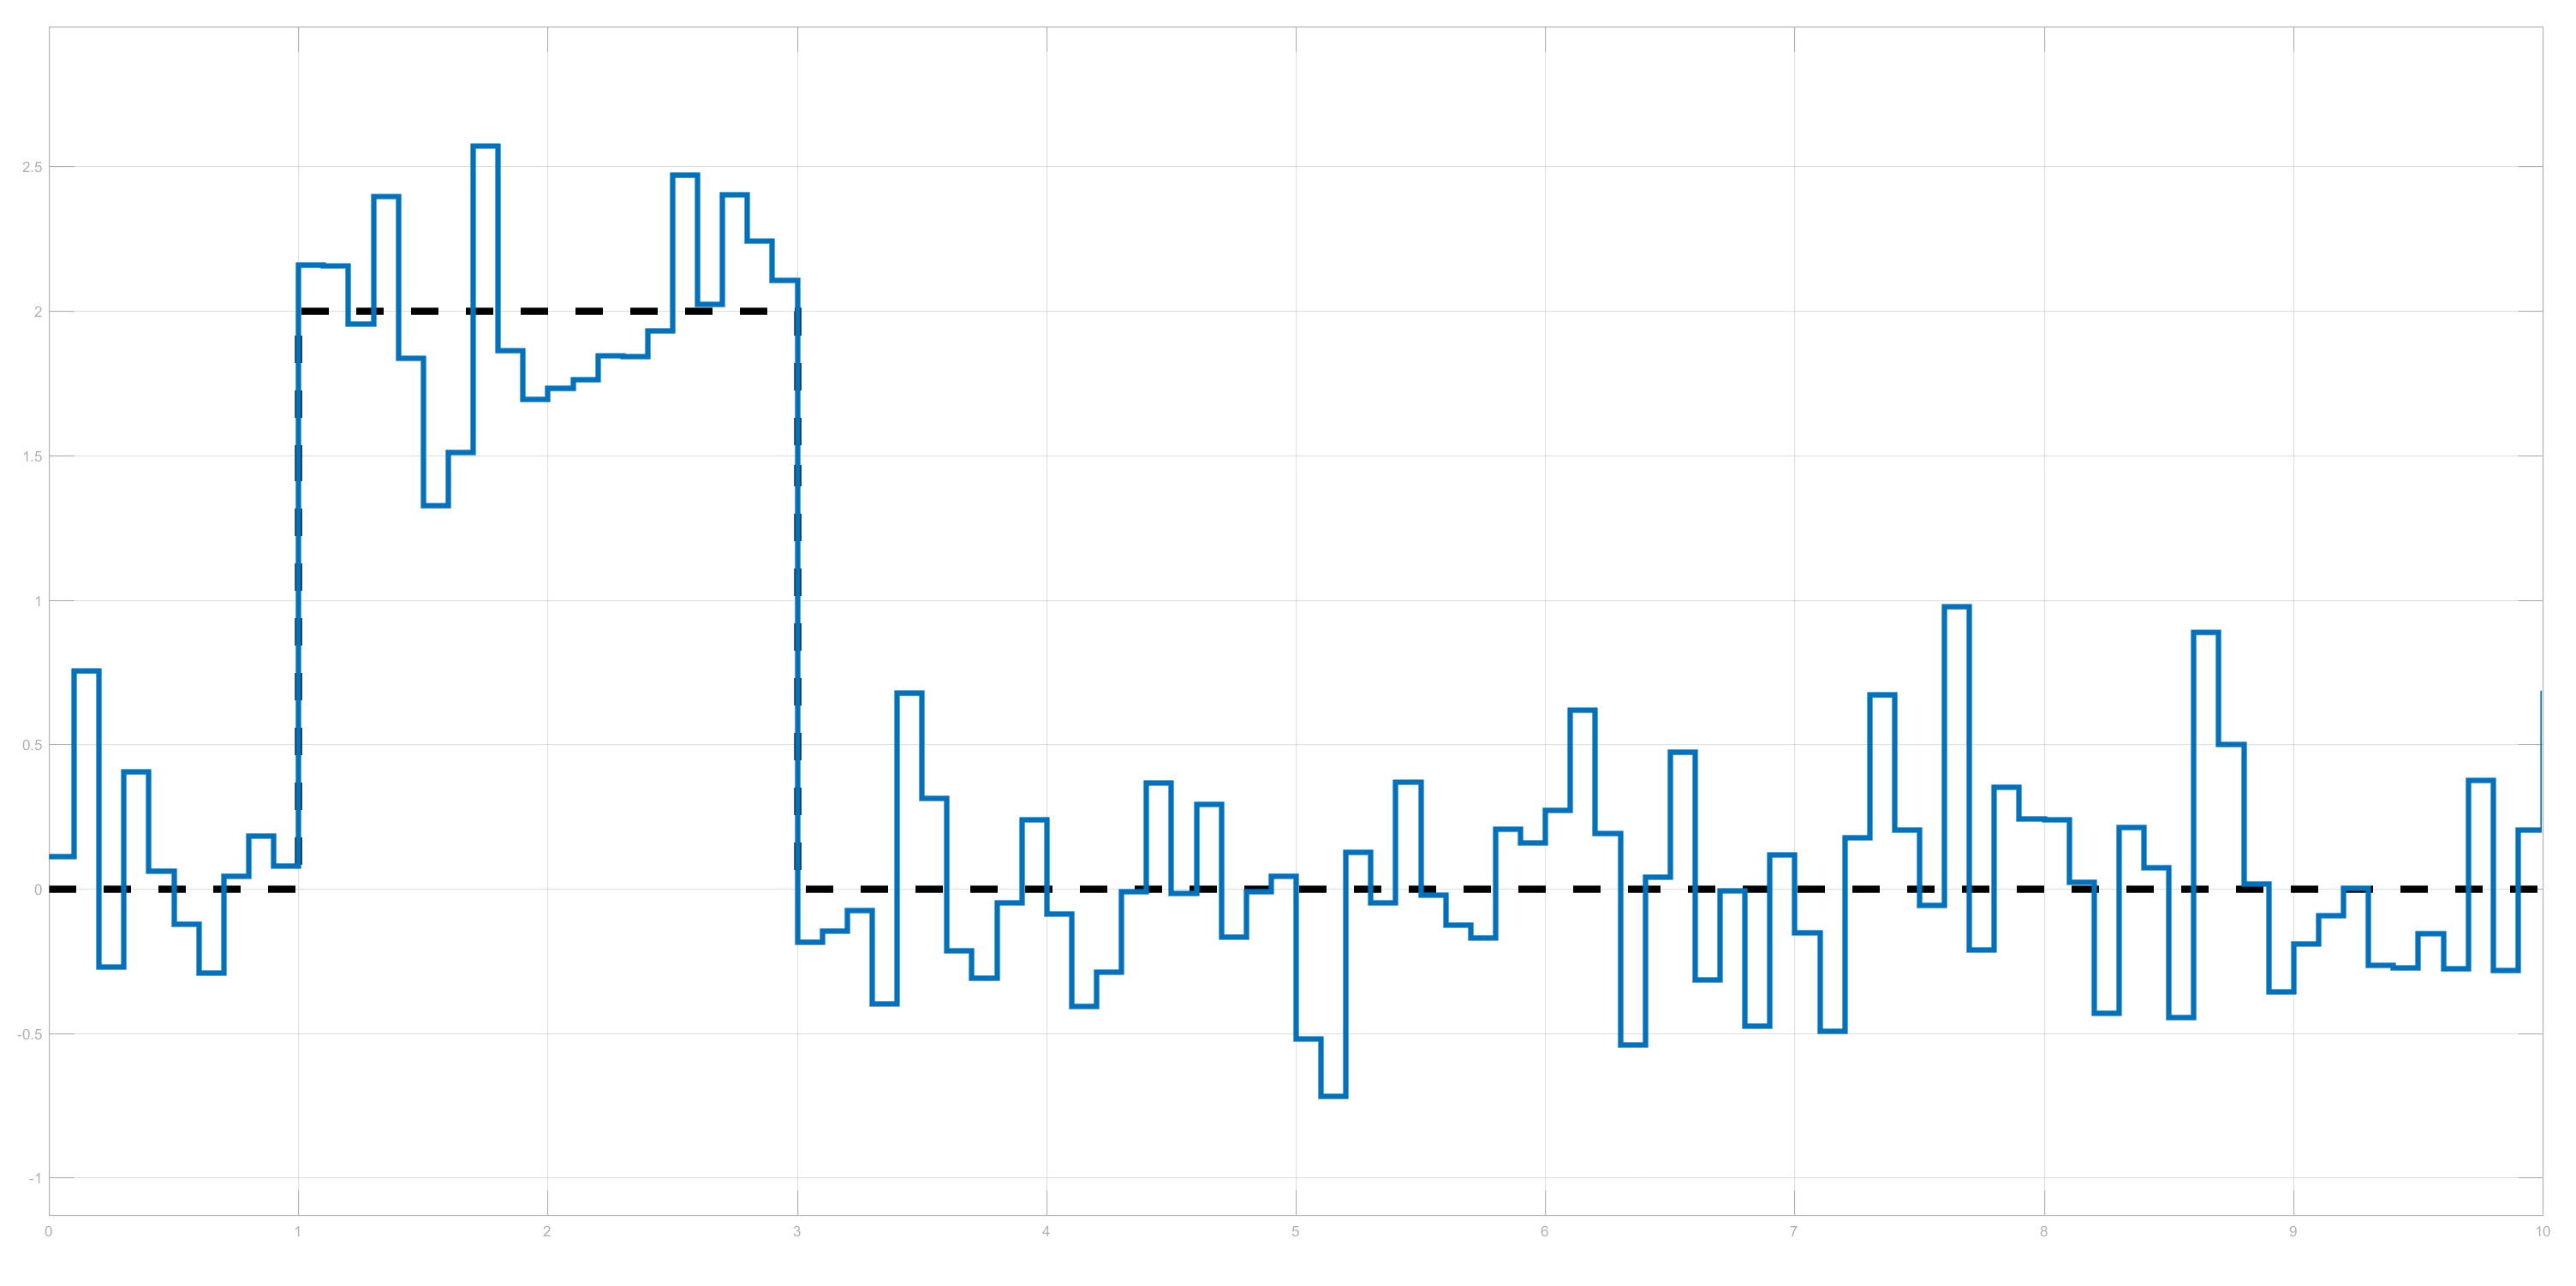
\includegraphics[scale=0.15]{Figuras/entrada}
  \caption{Señal de entrada perturbada.} 
\end{figure}

Adicionalmente, se introducen al sistema perturbaciones deterministas
de alta frecuencia con el fin de representar el posible deterioro de ciertas
componentes, pues si bien estos fenómenos son aleatorios, su impacto en el sistema
puede ser tratado localmente de manera determinista. Para ello se emplea por una señal computesta por la suma de señales senoidales de alta frecuencia.

Debido a la existencia de los ruidos y en busca de poseer un sistema más robusto, se diseña un filtro pasabajas de primer orden,
el cual, como su nombre lo indica, se caracteriza por permitir el paso de las frecuencias
más bajas y atenuar las más altas.

La literatura señala que la función de transferencia de dicho tipo de filtros
es de la forma~\cite{9780750300582}
\[
\frac{1}{\tau s + 1}
\]
donde $\tau $ es un parámetro temporal que depende de la frecuencia que se desea
filtrar, en particular para el problema planteado se decide escoger $\frac{1}{15}$.

Tanto en la Figura ~\ref{fig:filtro-angle} como en la Figura ~\ref{fig:filtro-c} se pude observar la
respuesta temporal del sistema excitado, con la entrada observada
en Figura ~\ref{fig:entrada-ruido}, perturbado y filtrado.

\begin{figure}[t]
  \label{fig:filtro-angle}
  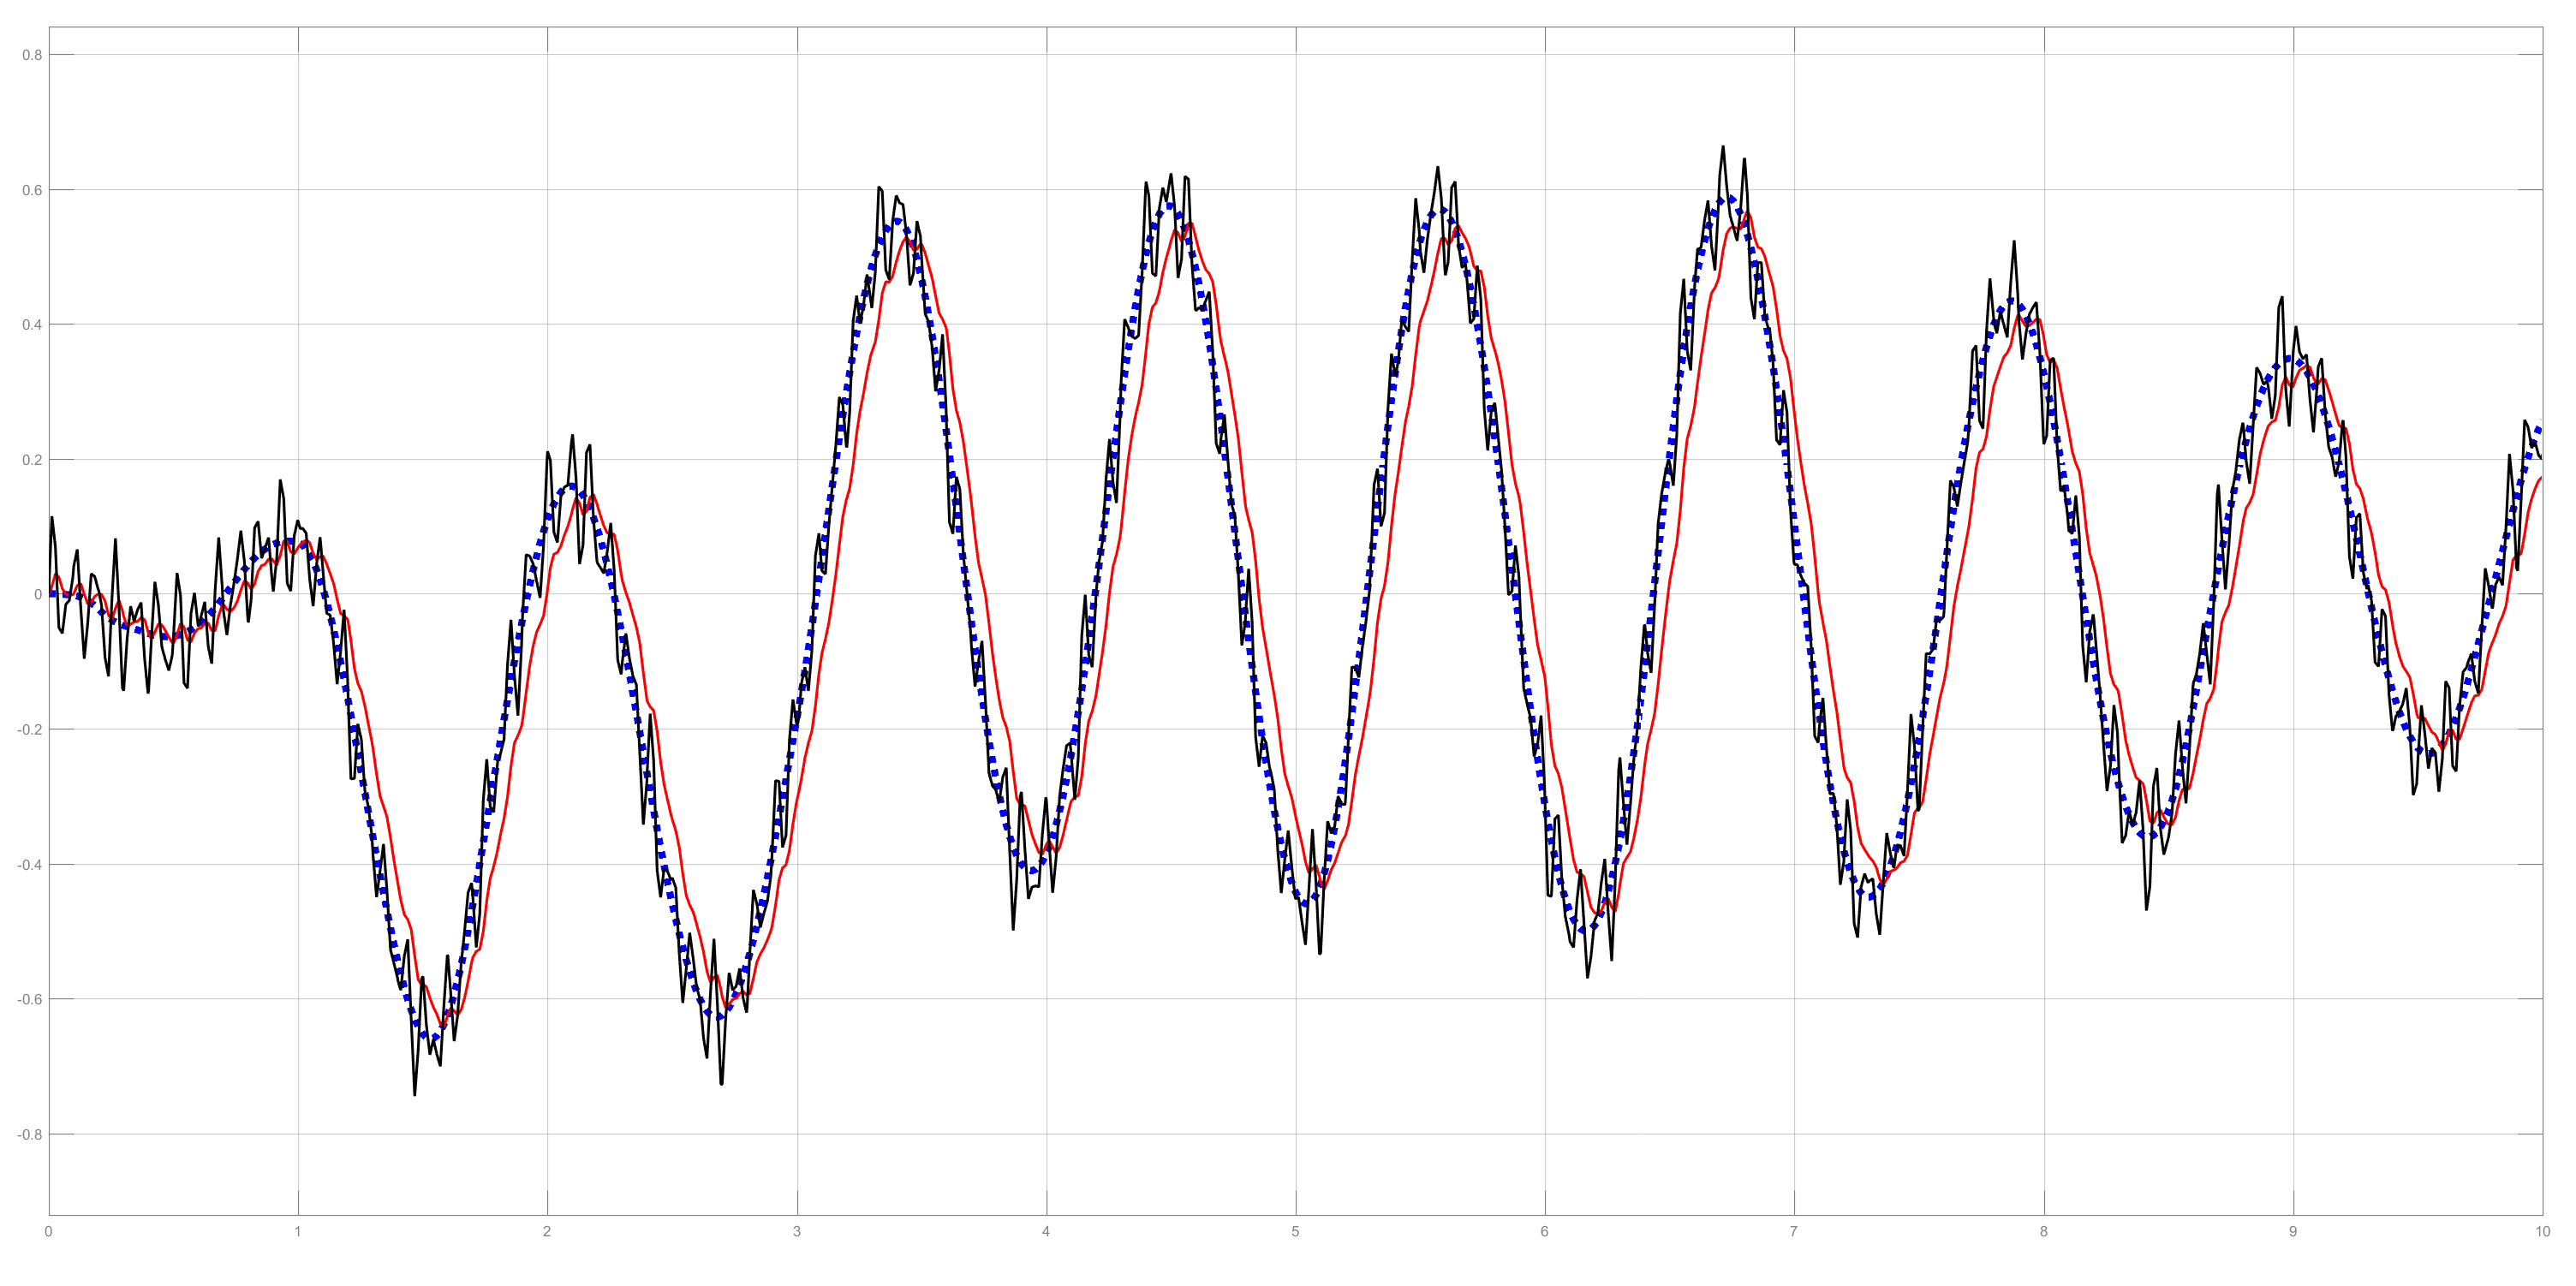
\includegraphics[scale=0.15]{Figuras/filtro-angle}
  \caption{Respuesta temporal del angulo perturbado y filtrado} 
\end{figure}

\begin{figure}[t]
  \label{fig:filtro-c}
  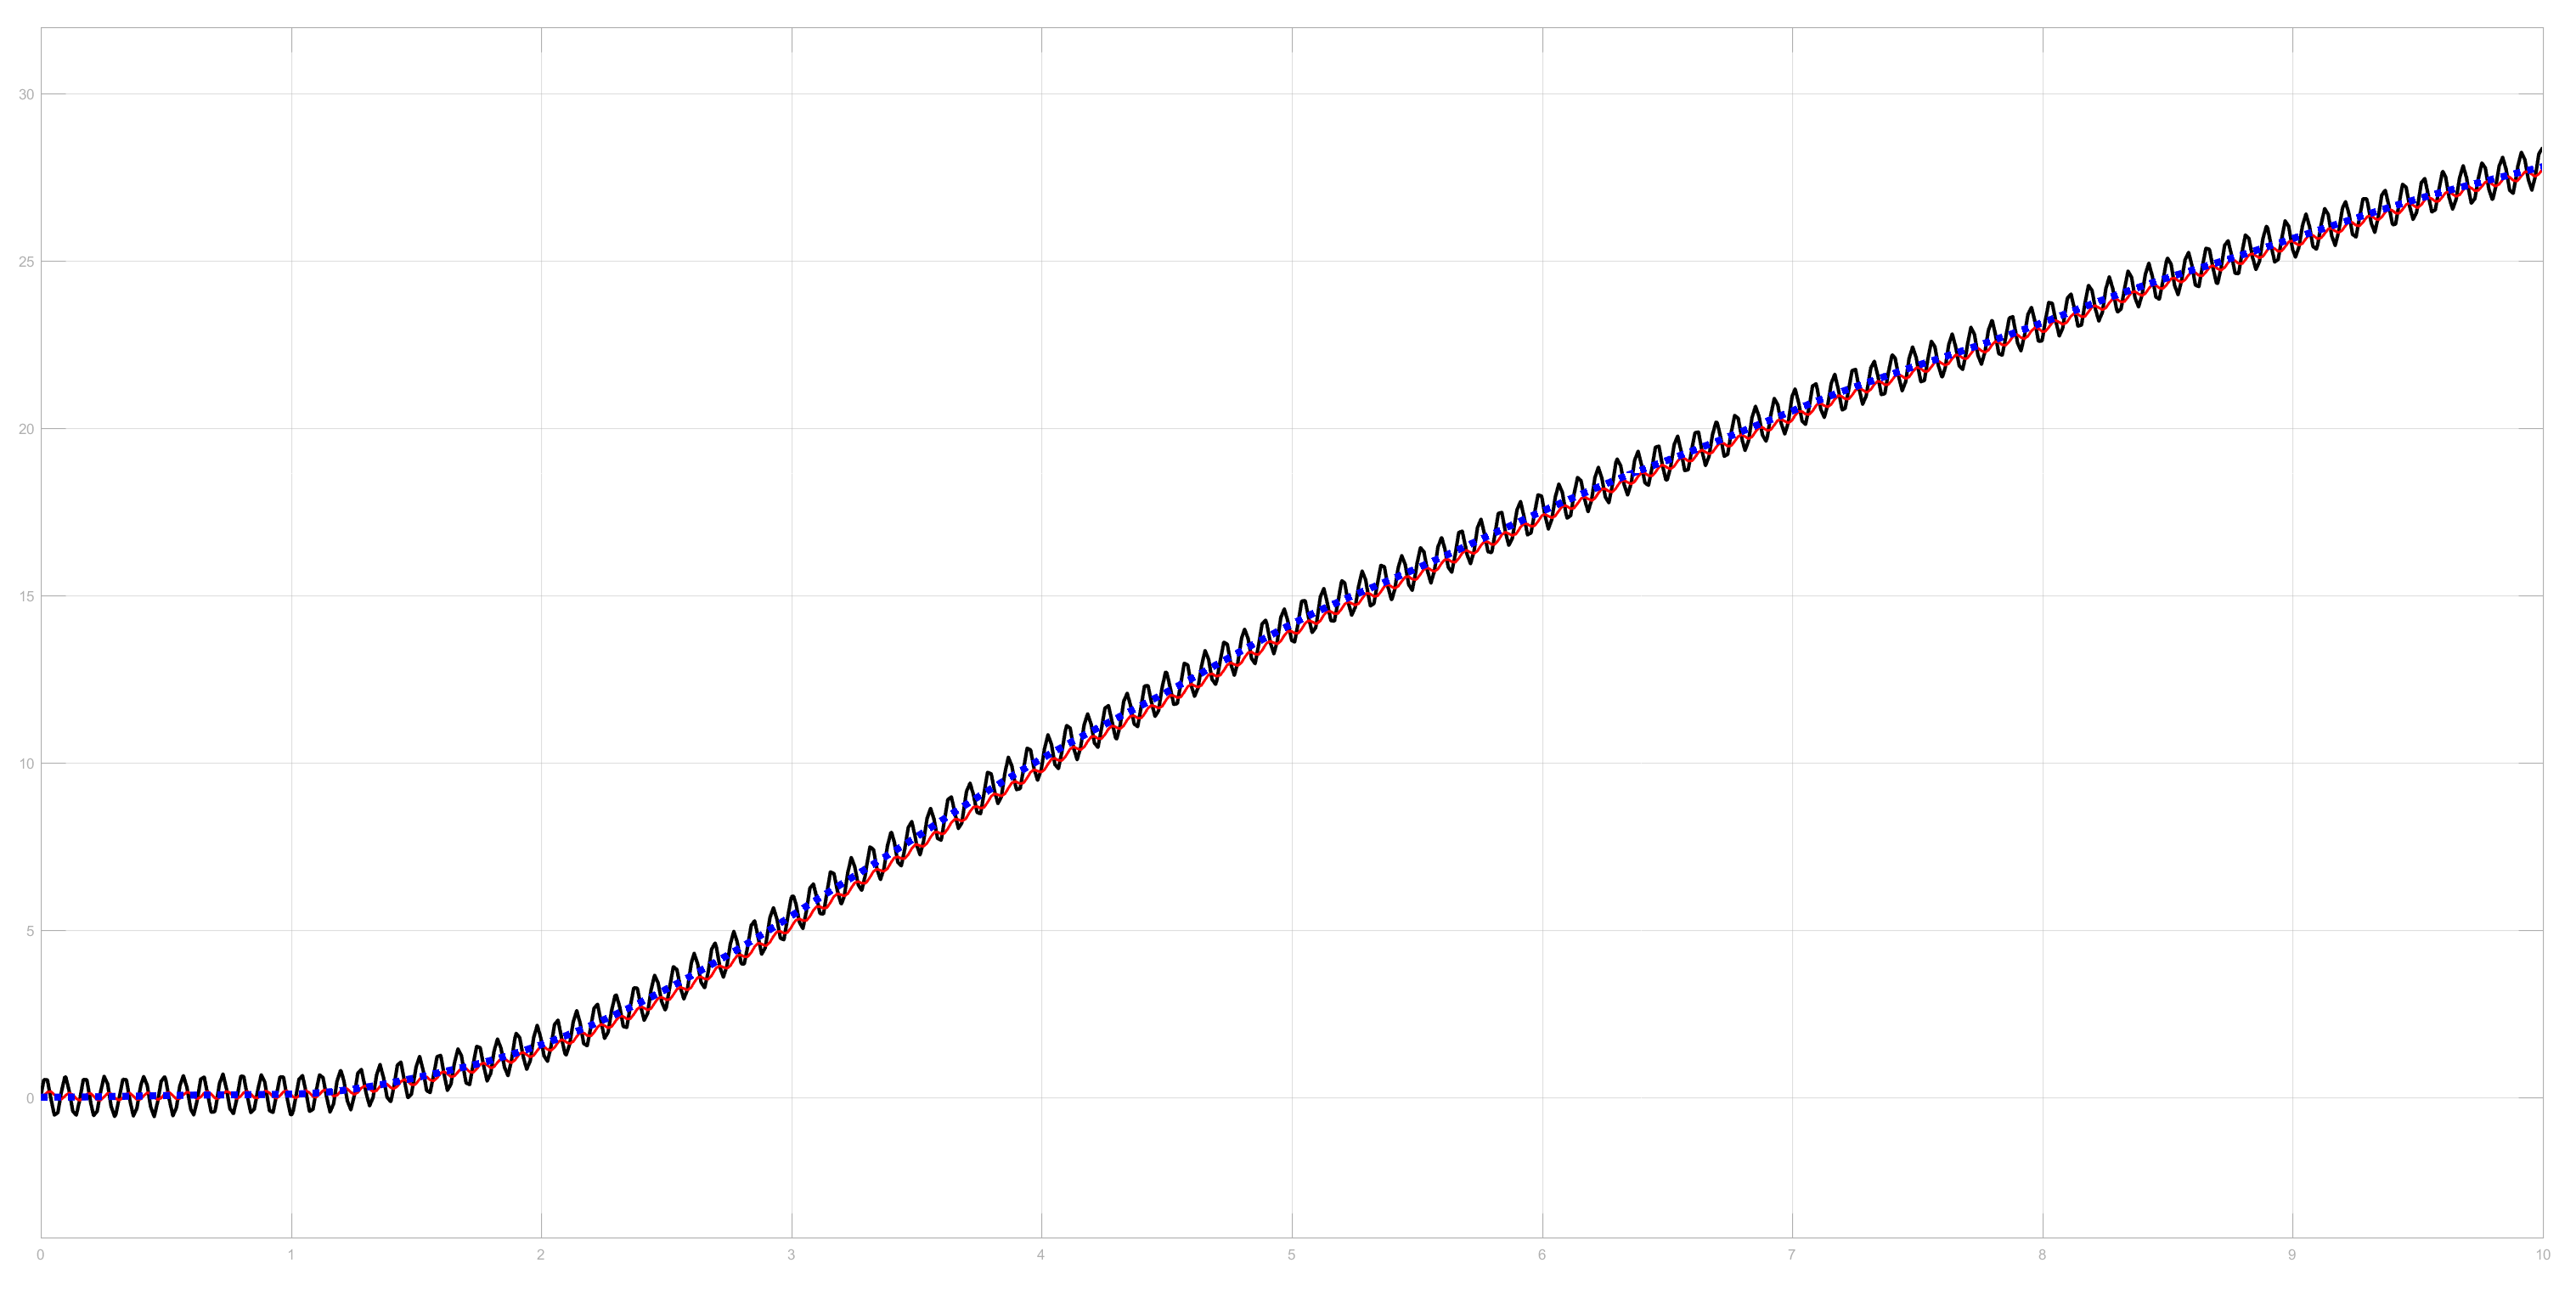
\includegraphics[scale=0.15]{Figuras/filtro-c}
  \caption{Respuesta temporal de la posicion perturbada y filtrada} 
\end{figure}

De las imagenes anteriores se puede deducir que los filtros son herramientas de gran importancia, ya que
permiten desechar los componentes indeseables y si bien estos generan pequeños retrazos que pueden comprometer
la estabilidad del sistema, pueden llegar a ser una herramienta fundamental en el diseño de cualquier planta
pues está siempre estará expuesta a diferentes fenomenos que puedan comprometer sus propiedades.